\section{Integration of the Model}

After training the model, it was crucial to integrate it smoothly into the existing workflow to avoid requiring the researcher to learn new software. The model was integrated into the Fiji software, which was already in use, instead of creating a new application.

The first step involved adding a new button to the Fiji interface, as shown in Figure~\ref{fig:enter-label-2}. Pressing this button triggers a Python script from the `StartupMacro`, with the path to the image being analyzed passed as an input argument. The script, stored in the Fiji application folder along with the macros and model parameters, loads the image and crops the lower part to remove irrelevant information. It then predicts a binary mask, processes it, and extracts the ten most relevant lines.

By default, another set of ten lines is added beneath the first set. The resulting data, containing the twenty lines, are saved in a zip folder. The path to this zip folder is then returned, and Fiji opens the folder to display the predicted lines to the researcher. If the researcher is dissatisfied with the predictions, they can modify the lines as needed.

\begin{figure}[ht]
    \centering
    \begin{subfigure}{0.45\textwidth}
        \centering
        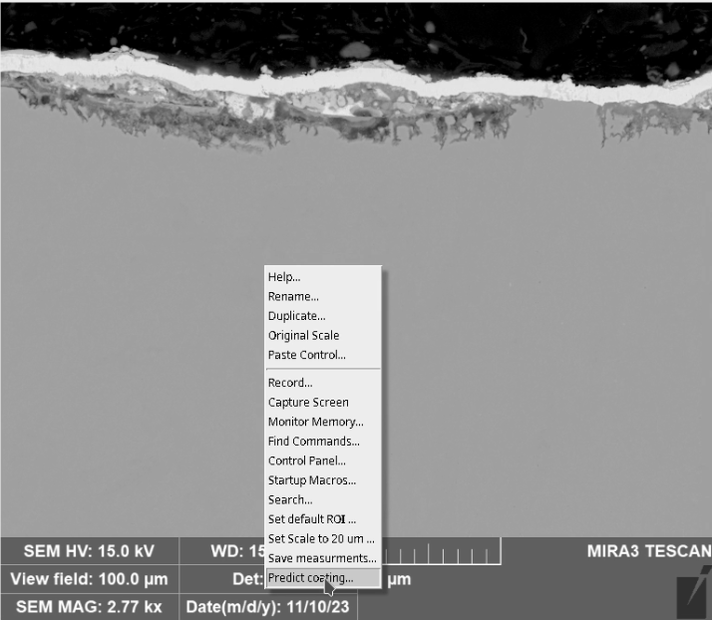
\includegraphics[width=\linewidth]{PICTURES/fiji/frame-002.png}
        \caption{Menu with \textit{Predict coating...} button}
        \label{fig:enter-label-2}
    \end{subfigure}
    \begin{subfigure}{0.45\textwidth}
        \centering
        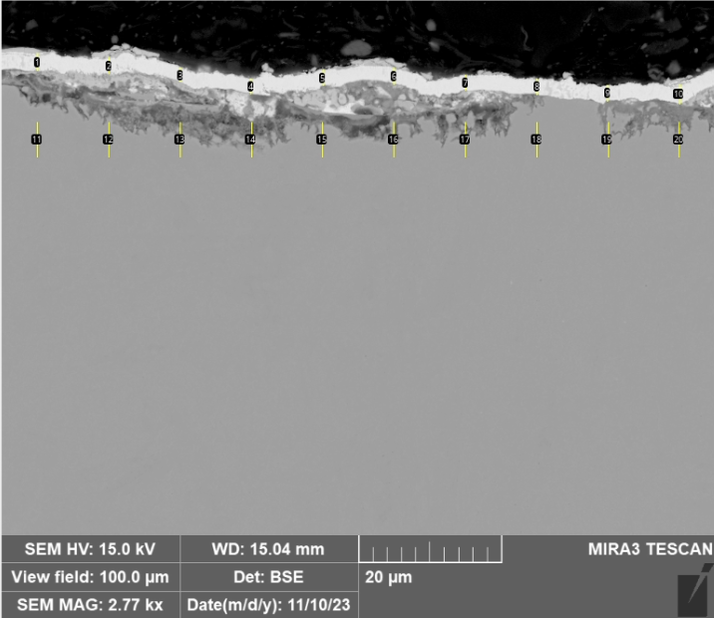
\includegraphics[width=\linewidth]{PICTURES/fiji/frame-003.png}
        \caption{Predicted lines}
        \label{fig:enter-label-3}
    \end{subfigure}
    \caption{Example workflow in Fiji}
    \label{fig:two-masks}
\end{figure}
\newpage
\section{Results - Time Experiment}

Following the model integration and the update to the Fiji setup, a time measurement study was conducted to assess time savings. Eight images were selected from four batches, with two images chosen from each batch. The experiment was designed as follows:

The first image in the set is measured manually, while the second is analyzed using the prediction model. In the first image from the first set, only the predefined default lines were used, simulating the first image in each batch where the researcher does not have lines similar to the coating. The first image from the second set used predefined lines from another image in the same batch. Since the images in each batch are similar, the researcher typically spends less time adjusting these lines. The third set followed the same approach as the second, but with an image where the model did not predict all the lines correctly. The fourth set included a challenging image with complex oxidation, where the model's predictions were less accurate, though the same approach as the second set was used on the first image.

The "Model" column in Table~\ref{tab:time-measurements} indicates whether the model was used for line prediction. The model was not used for the first image in each set but was used for the second image.

The "Predict" column shows the time from pressing the "Predict coating" button until the predicted lines were displayed, which took approximately 14 seconds, depending on the computer hardware. 

The "Measure" column represents the total time from starting the prediction (or manual measurement with predefined lines) to when the researcher finished editing. 

The "Add\_Excel" column reflects the time the researcher took from the start until adding the measurements to the Excel file. When using the model, the researcher worked with an updated version of Fiji, which included the improvements described in \textit{Fiji adjustments} (\ref{sec:1.2.2}). Consequently, Fiji, with the model, was also able to export to Excel faster.


\begin{table}[H]
\centering
\begin{tabular}{|l|l|l|l|l|}
\hline
\textbf{Type}           & \textbf{Model} & \textbf{Predict} & \textbf{Measure} & \textbf{Add\_Excel} \\ \hline
First Batch             & N             & /                & 01:12.00         & 01:30.00         \\ \hline
First Batch             & Y             & 00:14.00         & 00:28.00         & 00:38.44         \\ \hline
Normal                  & N             & /                & 00:57.32         & 01:26.00         \\ \hline
Normal                  & Y             & 00:14.00         & 00:25.20         & 00:38.34         \\ \hline
Model Wrong             & N             & /                & 01:09.00         & 01:32.00         \\ \hline
Model Wrong             & Y             & 00:14.00         & 00:57.32         & 01:10.00         \\ \hline
Hard Oxidation          & N             & /                & 01:05.00         & 01:26.00         \\ \hline
Hard Oxidation          & Y             & 00:14.00         & 00:45.24         & 00:59.00         \\ \hline
\end{tabular}
\caption{Time measurement results for four sets of images. All times are in min:s:ms.}
\label{tab:time-measurements}
\end{table}
\subsection{Time per one batch}

A theoretical batch of 30 images was considered for this experiment. It was assumed that the first image in the batch would take the longest to process, as is explained in \ref{sec:ManualProc}. Additionally, two images were expected to experience significant model errors, while two others presented challenging oxidation conditions. The time spent on measurement with the model was approximated as:

\[
\text{Time with model} = 28 + (25 \times 25) + (57 \times 2) + (45 \times 2) = 857 \text{ seconds} = \frac{857}{60} \approx 14.28 \text{ minutes}.
\]

The results of the time calculations are summarized in Table \ref{tab:time_comparison}.

\begin{table}[H]
    \centering
    \renewcommand{\arraystretch}{1}
    \begin{tabular}{|c|c|c|}
        \hline
        \textbf{Scenario} & \textbf{Time (seconds)} & \textbf{Time (minutes)} \\
        \hline
        Model - Measure & 857 & $\frac{857}{60} \approx 14.28$ \\
        \hline
        Manual - Measure & 1765 & $\frac{1765}{60} \approx 29.42$ \\
        \hline
        Model - Total & 2596 & $\frac{2596}{60} \approx 43.27$ \\
        \hline
        Manual - Total & 1246 & $\frac{1246}{60} \approx 20.77$ \\
        \hline
    \end{tabular}
    \caption{Comparison of time taken in different scenarios}
    \label{tab:time_comparison}
\end{table}

The percentage reductions in time are presented in Table \ref{tab:percentage_reduction}:

\begin{table}[H]
    \centering
    \renewcommand{\arraystretch}{1}
    \begin{tabular}{|c|c|}
        \hline
        \textbf{Scenario} & \textbf{Percentage reduction} \\
        \hline
        Reduction in measurement time & $\frac{29.42 - 14.28}{29.42} \times 100 \approx 51.5\%$ \\
        \hline
        Reduction in total time & $\frac{43.27 - 20.77}{43.27} \times 100 \approx 52.0\%$ \\
        \hline
    \end{tabular}
    \caption{Percentage reduction in measurement and total time}
    \label{tab:percentage_reduction}
\end{table}

Thus, using the model results in significantly faster processing times for measurement and saving results. Although these measurements are approximations, the results clearly demonstrate that the model improves the speed of the process.

\section{Results - Precision}

After the model was integrated into the workflow, data were collected from the research process. A total of 90 images were analyzed using the model. For each image, two folders were generated: one containing the predicted lines and another for the lines that could be manually adjusted by the researcher. The results from three separate batches are summarized below.

The first and second batches showed high accuracy, requiring minimal manual adjustments. However, the third batch exhibited reduced performance. This decline was attributed to the introduction of different types of layers. Notably, the model also detected the white oxidation layer above the coating layer, as shown in Figure~\ref{fig:ox}. This layer is visually similar to other structural layers, as seen in Figure~\ref{fig:three-images} (right image).

\begin{figure}[H]
    \centering
    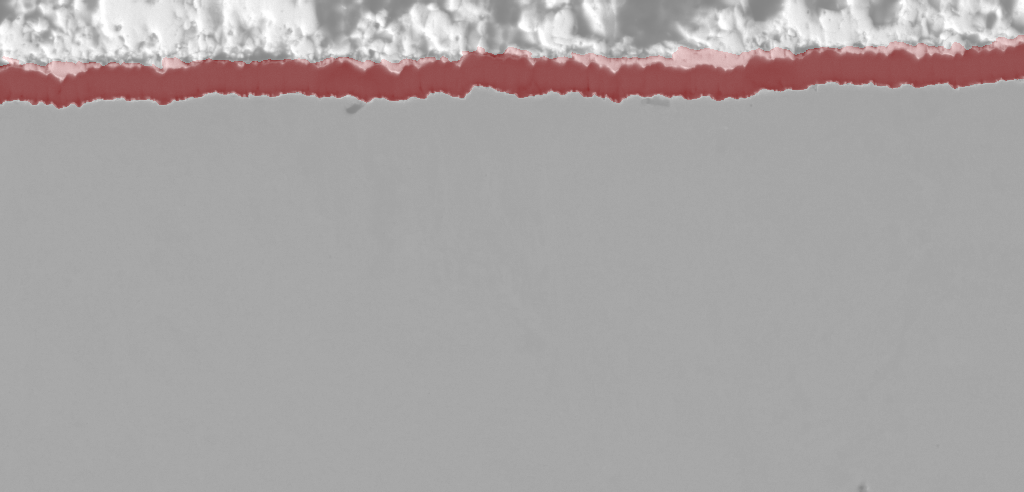
\includegraphics[width=0.5\linewidth]{PICTURES/aa.png}
    \caption{Image from the third batch, highlighting a poor prediction.}
    \label{fig:ox}
\end{figure}

These results suggest that the model performs well overall, requiring only minor adjustments in most of the cases. However, the findings also highlight the need to obtain a bigger dataset. The current dataset is still relatively small. These new data can be incorporated into the dataset using polygon labels, which can be efficiently created using automated scripts. After this, the model can be re-trained to make it more robust. This will create a feedback loop where labels can be generated faster, leading to a larger dataset, which in turn, after re-training, improves overall precision and results in time savings.

The precision of the model's predictions was evaluated by counting the number of points that required manual adjustment after the predictions were made. Table~\ref{tab:results} presents the summary statistics for the three analyzed batches.

\begin{table}[H]
    \centering
    \begin{tabular}{lcc}
        \toprule
        \textbf{Batch} & \textbf{Mean difference (pixel)}  & \textbf{Unchanged Points (\%)} \\
        \midrule
        1 & 1.11  & 93.3\% (560/600) \\
        2 & 0.57  & 97.3\% (584/600) \\
        3 & 5.58  & 22.7\% (136/600) \\
        \bottomrule
    \end{tabular}
    \caption{Analysis of model predictions across three batches.}
    \label{tab:results}

\end{table}

As shown in Table~\ref{tab:results}, the first two batches display a high percentage of unchanged points, indicating that the model's predictions are highly accurate. In contrast, the third batch shows a significantly higher mean difference and a lower percentage of unchanged points. This highlights the need for additional data to improve the model's performance.







\begin{comment}
\subsection{Evaluation}
To properly evaluate each model so they can be compared evaluation metrics need to be defined.  
\subsection{IoU}
IoU quantifies the overlap between the predicted mask and the actual layer, revealing how well the model captures the layer.  Equation 1 shows the mathematical formula for IoU. From the library torchmetrics, JaccardIndex can be imported. That is analogous to IoU. 
\subsection{    Average Start-End Differences }
This metric measures the average absolute difference between the start and end points of detected lines compared to researcher-marked lines (ground truth). Each image can have a maximum of 10 lines.  

If a researcher hasn't marked a line (resulting in NaN), the difference for both starts and endpoints is recorded as NaN in the results. 
\subsection{    Average Length DifferenceS }
This is the average length difference of the predicted 10 lines per mask and the ground truth. It penalizes the nan values the same way as 3.2. 
\subsection{    Mean Squared Error (MSE) of Differences }
The Mean Squared Error (MSE) of differences builds upon metrics 3.2 and 3.3. Unlike the mean absolute difference, MSE squares the errors before averaging them. This approach assigns greater weight to larger errors, making it more sensitive to outliers. Since large errors are particularly problematic in this project, MSE is a well-suited metric for evaluating the accuracy of line detections. 

\section{Connection to Fiji}
To integrate the trained model into Fiji, an existing startup macro was utilized. This macro opens and executes a Python script, which serves as an Application Programming Interface (API). The Python script begins by taking an image and the number of lines to be detected as input. It then uses a pre-trained model, represented by a .pth file, to predict a mask for the image. 

Following the prediction, the mask undergoes a three-stage post-processing procedure to eliminate noise and incorrect predictions. First, all white clusters within the predicted mask are converted into an array. The script then identifies clusters that touch both the left and right borders of the image—since such clusters are most common. If no such clusters are found, the script looks for the largest cluster that touches either the left or right borders. This step is particularly useful when intense oxidation occurs in the middle of the image. If neither of these criteria is met, the script selects the largest cluster available. 

Here are some images to demonstrate various types of postprocessing 

Once the mask is processed, it is sent to another function that generates the regions of interest (ROIs) that researchers need. This function uses a library to generate lines based on the first and last occurrences of white pixels in the mask, aligned with the y-axis at specific x-coordinates predefined by the researcher. If no lines are found, default lines are generated. Additionally, a second set of lines is produced below the first 10 predicted lines on default places. This second set is important because researchers are also measuring oxidation on minority samples when it occurs. 

The generated lines are then saved into a zip file, and the path to this zip file is communicated back to the Fiji application. The Fiji application then automatically opens the zip file, presenting the lines to the user. This entire process is hidden from the user; they only need to click on the model button and wait for a short duration, depending on the type of computer, after which the lines will appear. researchers can inspect these lines and, if necessary, edit them, just as they were able to do before. 
\end{comment}